%%%%%%%%%%%%%%%%%%%%%%%%%%%%%%%%%%%%%%%%%%%%%%%%%%%%%%%%%%%%%%%%%%%%%%%%%%%
%                                                                         %
%                      Pulse Height Discrimination                        %
%                                                                         %
%%%%%%%%%%%%%%%%%%%%%%%%%%%%%%%%%%%%%%%%%%%%%%%%%%%%%%%%%%%%%%%%%%%%%%%%%%%
Generally, two methods are available for discrimination; 1) pulse shape discrimination and 2) pulse height discrimination.
In pulse shape discrimination the different decay times between the neutron and gamma pulses are exploited to develop a metric that allows for the classification of the pulse, and preforms best when the pulses are noticeably different.
Pulse height discrimination is based on setting a pulse height discriminator that acts as a partition between two classes of pulses.

A pulse height discriminator may be set by hardware electronics or by software.
A mathematical lower level discriminator (MLLD) is then introduced to clarify the determination of what discriminator setting will be necessary to achieve a given intrinsic efficiency criteria.
The intrinsic efficiency for a given MLLD is determined for a sample by first determining the photon fluence over the sample (usually by a MCNPX calculations, these calculations are explained in \autoref{chap:DetChar}).
The recorded spectra is then normalized the photon fluence to determine the count rate per incident photon per channel.
As the intrinsic efficiency is defined as the count per incident quanta of radiation, the spectra needs to be integrated from the channel number represented by the MLLD to the end of the spectra over the channels to determine the count rate.
By summing only the counts that are above the discriminator represented as the MLLD these counts are then discarded from the analysis.
A formulation of the MLLD is presented in \eqref{eqn:MLLDFormulation},
\begin{align}
	\epsilon_{\gamma,int}\left(MLLD\right) &= \frac{\int_{MLLD}^{\infty}p(x)dx}{\Phi}
  \label{eqn:MLLDFormulation}
\end{align},
where \definevar{$p(x)$}{spectra as a function of channel number} and \definevar{$\Phi$} is the incident gamma flux.
By computing the gamma intrinsic efficiency as a function of the MLLD, one only needs to find what MLLD corresponds to having a intrinsic efficiency of less than one in a million.

A sequence of polystyrene films (10\% by weight enriched LiF) were fabricated by Dr. Mabe and analyzed for their ability to achieve different gamma intrinsic efficiencies in the MLLD framework.
These measurements and calculations, presented in \autoref{fig:GammaIntEffMLLD}, demonstrate the utility of the MLLD.
This figure shows, as expected, that increasing the MLLD causes a lower intrinsic efficiency as counts below the MLLD are discarded.
Thicker films, where more energy is deposited and thus produce more photons, require higher MLLD settings in order to achieve the same level of discrimination as their thinner counter parts.
\begin{figure}
  \centering
    \includegraphics[width=\textwidth]{PS_intEffMLLD}
  \caption[Intrinsic efficiency achieved at various discriminator settings]{Gamma intrinsic efficiency versus the pulse height discriminator setting (MLLD) to achieve the corresponding level of discrimination in 10\% loaded polystyrene. It is observed that there is a change in the shape of the curves reflecting the increased fraction of energy deposition in thicker films relative to the thinner films.}
  \label{fig:GammaIntEffMLLD}
\end{figure}

A pulse height discriminator to achieve the necessary gamma discrimination will not be without cost, however, due to an overlap between the neutron and gamma pulse height distributions.
For example, the calculated gamma intrinsic efficiency for six polymeric films along with the neutron response of two of the films is shown in \autoref{fig:GammaIntrNeutronCounts},
In order to achieve an intrinsic efficiency of less than \num{1E-6} the MLLD must be set above 2,000 channels, discarding a large majority of the neutron counts.
It is observed that if the films are thin enough (less than \SI{150}{\um}) it is possible to have a significant count rate above the mathematical lower level discriminator necessary for the pulse height discrimination of one in a million.
This is seen by the \SI{50}{\um} film and the \SI{150}{\um} film having the tail of their neutron spectra above the pulse height discriminator necessary for an intrinsic efficiency of \num{1E-6}.
\autoref{tab:FractionCRGamma} shows the fraction of neutron count rate that is above the MLLD necessary for $\epsilon_{int,\gamma n} \le \si{1E-6}$.
Films less than \SI{50}{\um} have over 16\% of the counts above the necessary discriminator setting, while thicker films have have a factor of 10 less.
\begin{figure}[ht]
    \centering
    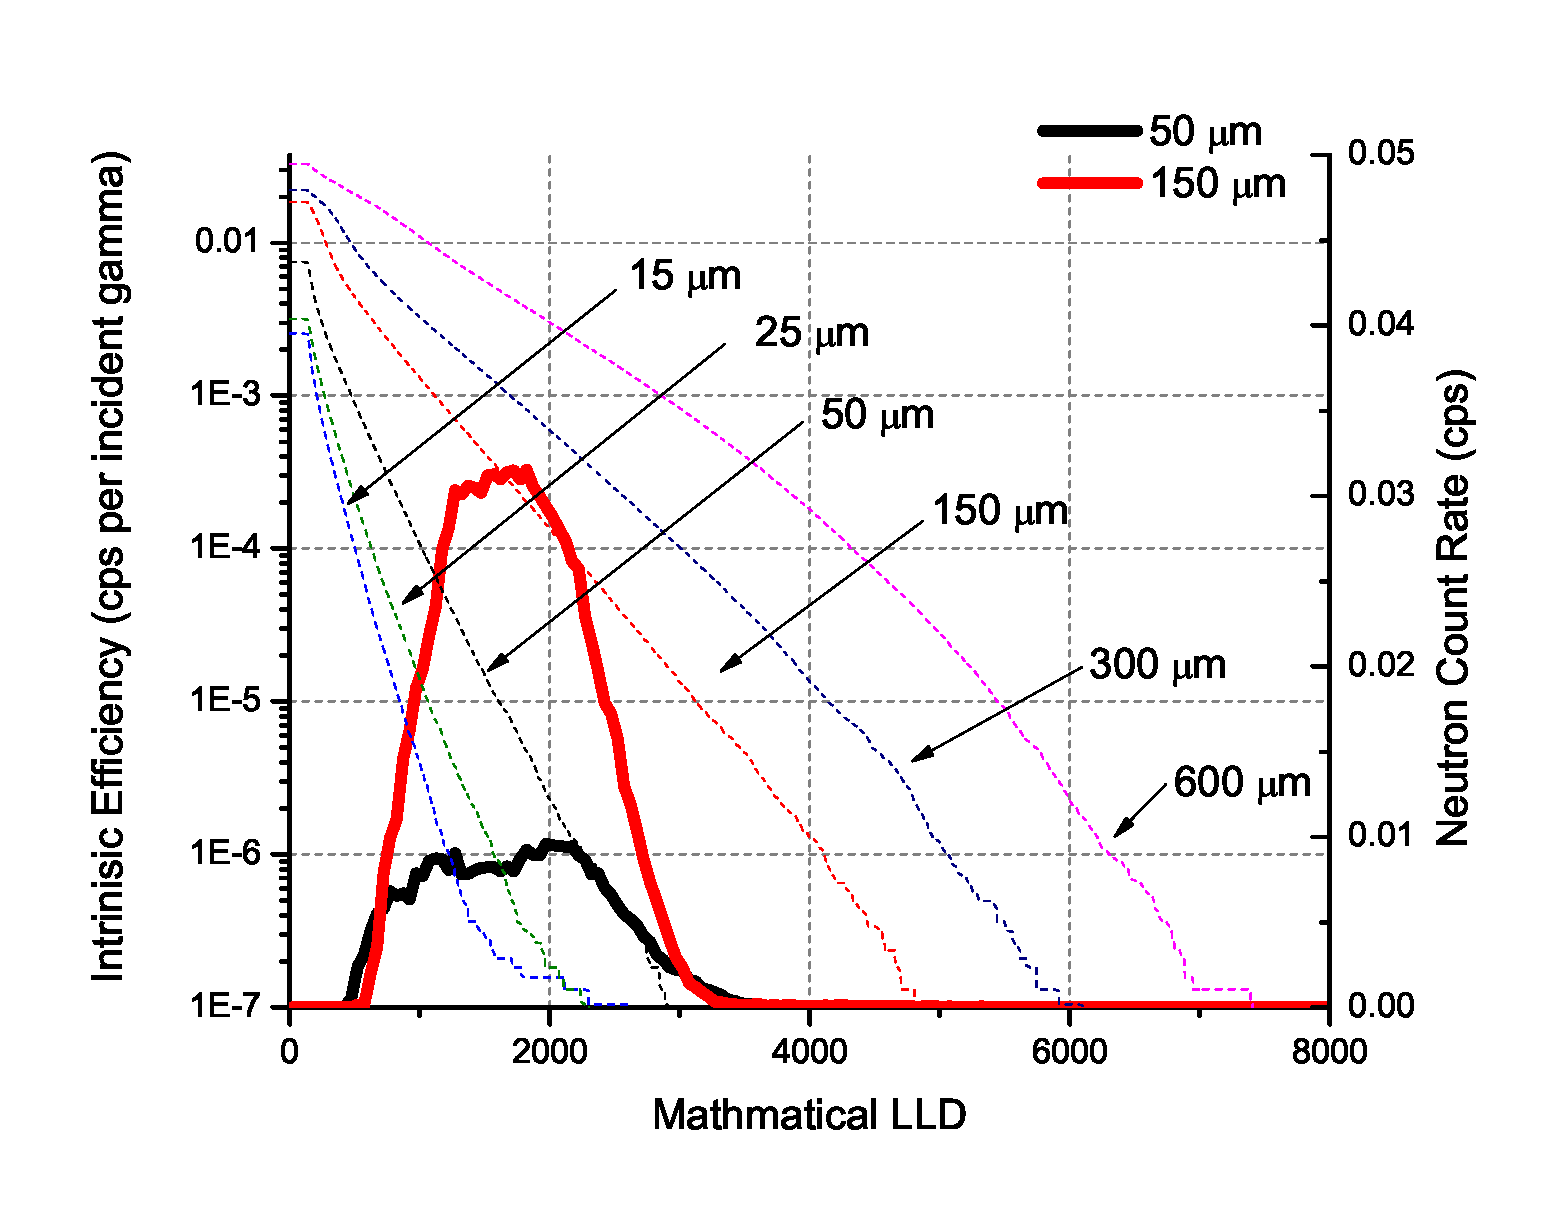
\includegraphics[width=\textwidth]{PS_IntEff_LiF20_PPO5}
    \caption[PS Gamma intrinsic efficiency and neutron count rate]{Gamma intrinsic efficiency (dashed lines) plotted against neutron counts (solid). The gamma spectra has been normalized by the number of incident photons upon the sample, while the neutron spectra has not. The material is polystyrene loaded with 10\% \iso[6]{LiF}.}
    \label{fig:GammaIntrNeutronCounts}
\end{figure}
\begin{table}
    \caption{Fraction of Neutron Count Rate Above Discriminator Setting in 10\% loaded polystyrene}
	\centering
	\begin{tabular}{c | c}
	Thickness & Neutron Fraction \\
	\hline
	\hline
	\SI{15}{\um} & 0.21 \\
	\SI{25}{\um} & 0.30 \\
	\SI{50}{\um}  & 0.16 \\
	\SI{150}{\um}  & 0.009 \\
	\SI{300}{\um}  & 0.002 \\
	\SI{600}{\um}  & 0.002 \\
	\end{tabular}
  \label{tab:FractionCRGamma}
\end{table}
In addition it is observed in \autoref{fig:GammaIntrNeutronCounts} that for neutrons, thicker films only enhance the resolution of the film and do little to increase the light yield, as most of energy from a neutron event is captured in the film.
